\documentclass{article}

\usepackage[margin=1in]{geometry}
\usepackage{graphicx}
\usepackage{enumitem}
\usepackage{parskip}
\usepackage[usenames]{xcolor}
\usepackage{listings}
\usepackage{hyperref}
\usepackage{caption}

\lstdefinelanguage{vns}
{keywords={add,sub,mul,div,and,orr,xor,nan,clz,cnt,lsr,lsl,abs,rnd,cmp,jiz,jnz,jgz,jlz,jge,jle,biz,bnz,bgz,blz,bge,ble,blx,ldr,str,pop,psh,
           who,wht,qcs,qct,qbp,qck,gnd,whr,dst,cvr,ded,sht,dir,wlk,crl,swm,cap,rtt,hid,say,rad,yel,ear,die,nrt,nre,est,soe,sot,sow,wst,nrw,
           wcs,wct,wbp,wcl,tcs,tct,tbp,tcl,pnt,ccs,cct,cbp,ccl,ucs,uct,ubp,ucl,dcs,dct,dbp,dcl,mcs,mct,mbp,mcl,rcs,rct,rbp,rcl,tim,dly,adv,
           ask,plz,beg,gvl,kmk,sac,bom,air,sum,hak,emp,all,rmt,rsn,res,ref,rms,rmf,rss,rsf,rrs,rrf,wmt,wsn,wes,wef,wms,wmf,wss,wsf,wrs,wrf,
           wtg,rtg,wsg,rsg,wfg,rfg,itf,fad,fsu,fmu,fdv,cel,flr,sin,cos,tan,pow,asn,acs,atn,log,fcp,mle,set,css,cfs,wss,wfs,gup,sup,
           cam,unc,hip,nmr,ist,tgt,lie,mor,
           wir,cut,snd,dig,
           mlf,
           run,hit},
 sensitive=false,
 comment=[l]{;},
}

\newcommand{\vnscode}[1]{\colorbox{lightgray}{\lstinline[language=vns]{#1}}}

\newcommand{\UT}{\lower-0.5ex\hbox{u}\kern-1.1ex T}
\newcommand{\RT}{\lower-0.5ex\hbox{r}\kern-0.65ex T}
\newcommand{\RP}{R\kern-0.85ex P}

\title{Von Neumann Standing -- Instructions}
\date{\today}
\author{Louis A. Burke}

\begin{document}
\maketitle
\clearpage
\tableofcontents
\clearpage
\listoftables
\clearpage

\section{Introduction}

A game of Von Neumann Standing is played between two sets of programs. It
simulates a wartime battle over a river. The winner is whichever team captures
the enemy base.

\subsection{Units}

Each team consists of 11 units. Each unit runs its own program to determine its
actions. The team with the smartest programs will win the game.

The first unit is the captain. The captain isn't as effective in combat as the
rest of the team, but can defend itself. Its primary role is to requisition
additional resources and coordinate the movements of its team.

The second unit is the mortar. The mortar has to spend time setting up and
tearing down its weapon in order to fire it or move. While largely incapable of
defending itself, the mortar can drop area of effect shells on units from any
distance, ignoring cover.

The third unit is the sniper. The sniper can camouflage itself to make it
difficult for other units to see it. It can fire accurate bullets from afar and
through cover to dislodge the hardiest of units. You can be sure the sniper will
be a prime target for the enemy if spotted.

The fourth and fifth units are the engineers. They can construct defenses such
as cover and barbed wire. They are not the best in combat, but can tear through
enemy defenses with ease.

The sixth and seventh units are the machine gunners. Like the mortar they have
to setup and tear down their weapons in order to fire and move. Once setup
however, they can protect themselves well with the most powerful short-range
weapon in the game. It is unwise for any unit to approach a setup machine gun,
but mortars and snipers can sometimes take them on.

The eighth and ninth units are the scouts. They can move faster than any other
unit. While not very effective from afar, their shotgun will make short work of
nearby enemies. Additionally they can spot camouflaged snipers and have extra
visibility. The scouts can maintain constant communication with their sniper to
call in prospective targets.

The tenth and eleventh units are the riflemen. They are the primary soldiers of
the squad. Their relative expandability makes them the main offensive unit. They
can respond to support requests and offer tactical information to the rest of
the squad.

\subsection{Upgrades}

Each unit can upgrade its processor in order to execute its code faster. There
are four systems to be upgraded. The cache can be upgraded in both size and
algorithm. The branch predictor can be upgraded to make branches faster. Finally
the clock rate of the processor itself can be upgraded.

\subsection{Map}

The game is played on a 32 by 16 grid, with a team at either end. Separating the
teams is a large river. The river provides no cover, and nothing can be built on
it, nor setup on it. Both captains have the river marked for air strikes, so it
is unwise to leave any unit in it for long.

\clearpage

\section{Rules}

\subsection{Resources}

The game has only two resources. The first is the implicit resource of time. The
game operates on a universal clock cycle. One iteration of this cycle is
referred to as a \textit{Universal Tick} or \UT. However, each unit does not
execute an instruction every universal tick. Instead each of their
\textit{Relative Ticks} or \RT\ happen only on some of the universal ticks
(depending on CPU speed).

On top of time there is an explicit resource shared by each member of a team.
These are the team's \textit{Resource Points} or \RP. On each \UT\ each team
gains one \RP. \RP\ can be spent on upgrades and munitions.

\subsection{Shooting}

Each unit uses a different weapon. Different weapons take a different amount of
time to fire. The fire rate depends on the distance to the target, the cover the
target is behind, and the weapon being fired.

Each weapon has a base fire rate, a precision, and an accuracy.

The precision of a weapon applies to the distance of the shot, while the
accuracy applies to the cover that must be shot through. Cover directly in front
of the shooter does not count.
% Thought: maybe make units have to stand IN cover?

The exact formula for a weapon's firetime is:

$$t=b+pd+ac$$

Where $t$ is the time the shot takes in \RT, $p$ is the weapon's precision, $d$
is the distance to target, $a$ is the accuracy of the weapon, $c$ is the cover
between the shooter and the target.

The parameters of the weapons are:

\begin{minipage}{\textwidth}
\captionof{table}{Weapon Parameters}
\centering
\begin{tabular}{|l|l|c|c|c|r|}
    \hline
        Unit Name &
        Weapon Name &
        Base Rate ($b$) &
        Precision ($p$) &
        Accuracy ($a$) &
        Cost \\ \hline
    Captain & Pistol & 1 & 16 & 64 & 32 \RP \\ \hline
    Sniper & Sniper Rifle & 64 & 2 & 0 & 64 \RP \\ \hline
    Sniper & Hip Shot & 4 & 4 & 16 & 64 \RP \\ \hline
    Rifleman & Rifle & 4 & 4 & 16 & 64 \RP \\ \hline
    Engineer & Light Machinegun & 8 & 8 & 32 & 32 \RP \\ \hline
    Machinegunner & Machinegun & 1 & 8 & 64 & 64 \RP \\ \hline
    Scout & Shotgun & 8 & 16 & 4 & 64 \RP \\ \hline
    Mortar & Shell & 512 & 0 & 0 & 256 \RP \\ \hline
\end{tabular}
\end{minipage}

\subsection{Terrain}

There are six types of terrain in the game. The most common kind is open grass.
Open grass provides no cover but can be built upon by engineers. Wire is one of
the structures that can be built by engineers. It does not provide cover but
does impede unit movement. Cover can also be built by engineers. It doesn't
obstruct movement but does provide cover.

In the middle of the map is the river. Water tiles severely obstruct movement
and provide a sense of negative cover. Beach tiles similarly don't provide
cover, but movement is easy on them. Both water and beach tiles share a couple
properties. First nothing can be built on them, nor can units set up on them.
Additionally they do not count as increased distance for weapon shots, so a unit
on the shore can see all other units in or on the river as if they were right
next to them.

\section{Environment}

Each team's code runs it its own environment, with each unit running on their
own virtual machine. Each unit has 32 registers. The first 16 are the same for
each unit, while the second 16 are unit-specific. Additionally each unit has 1
megabyte of memory to run their code on.

\subsection{Command Layout}

The assembly language commands all take one of two forms.

The first form is the three-register command. For example \vnscode{add r1, r2,
r3} adds the values of registers 2 and 3 and stores the result in register 1.
These instructions leave 10 bits for a signed immediate value. This value is
accessible from register 12.  The assembler thus allows you to replace one
register with a 10-bit signed integer. This makes a common way to load a
register with a value to use \vnscode{add r1, r0, 10; Load 10 into r1}.

The second form is the single-register command. For example \vnscode{bnz r1,
123} will jump to address 123 if r1 is non-zero. These immediate values
typically refer to addresses, therefore it is common to use labels to refer to
them. These are any identifiers followed by a colon.

\subsection{Timing}

Different instructions take a different number of CPU cycles to complete. Using
efficient instructions can get your units to react faster.

\subsection{Specifics}

This section indicates some of the specifics of the game. Things such as integer
representations of concepts and formal definitions of terms are described.

\subsubsection{Directions}

This table indicates the codes for each direction. North is always towards
decreasing Y values and East is always towards increasing X values (relative to
your team's coordinate system).

\begin{minipage}{\textwidth}
\captionof{table}{Direction Codes}
\centering
\begin{tabular}{|c|c|c|}
    \hline North-West (8) & North (1) & North-East (2) \\ \hline
    West (7) & & East (3) \\ \hline
    South-West (6) & South (5) & South-East (4) \\ \hline
\end{tabular}
\end{minipage}

\subsubsection{Terrains}

This table indicates the codes for each terrain type.

\begin{minipage}{\textwidth}
\captionof{table}{Terrain Codes}
\centering
\begin{tabular}{c|c|c|c|c|c}
    Grass & Wire & Cover & Beach & Water & Base \\ \hline
    1 & 2 & 3 & 4 & 5 & 6
\end{tabular}
\end{minipage}

\subsubsection{Units}

This table indicates the codes for each unit type. Different codes refer to
different team's units.

\begin{minipage}{\textwidth}
\captionof{table}{Unit Codes}
\centering
\begin{tabular}{|c|c|c|}
    \hline Unit & Friendly ID & Enemy ID \\ \hline
    Captain & 1 & -1 \\ \hline
    Mortar & 2 & -2 \\ \hline
    Sniper & 3 & -3 \\ \hline
    Engineer (SS) & 4 & -4 \\ \hline
    Engineer (FS) & 5 & -5 \\ \hline
    Machinegunner (SS) & 6 & -6 \\ \hline
    Machinegunner (FS) & 7 & -7 \\ \hline
    Scout (SS) & 8 & -8 \\ \hline
    Scout (FS) & 9 & -9 \\ \hline
    Rifleman (SS) & 10 & -10 \\ \hline
    Rifleman (FS) & 11 & -11 \\ \hline
\end{tabular}
\end{minipage}

\subsubsection{Nearest}

The term nearest is used often in the game. Given the nature of the coordinate
system it is not clear what exactly the term implies.

In the game whenever a nearest computation is made a spiraling search pattern is
performed around the target square. This pattern can be visualized as:

{\centering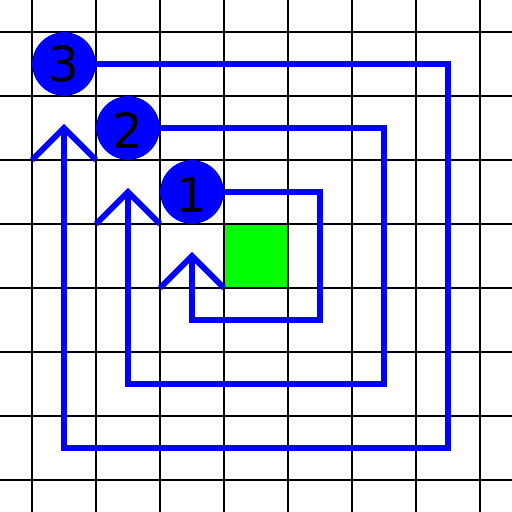
\includegraphics[width=0.5\textwidth]{res/nearest.png}\par}

This pattern is extended outwards indefinitely to cover the entire map aside
from the search square itself.

\section{Arithmetic Operations}

The assembly language used in this game contains many of the typical
arithmetic instructions one might see in a traditional assembly language. These
instructions are summarized below.

\begin{minipage}{\textwidth}
\captionof{table}{Arithmetic Operations}
\centering
\begin{tabular}{|c|c|l|l|}
    \hline \vnscode{CODE} & Instruction Name & Description & Time \\ \hline
    \vnscode{ADD a, b, c} & Add & Adds b and c, storing the result in a. & 1 \\ \hline
    \vnscode{SUB a, b, c} & Subtract & Subtracts c from b, storing the result in a. & 1 \\ \hline
    \vnscode{MUL a, b, c} & Multiply & Multiplies b and c, storing the result in a. & 4 \\ \hline
    \vnscode{DIV a, b, c} & Divide & Divides b by c, storing the result in a. & 8 \\ \hline
    \vnscode{AND a, b, c} & Bitwise AND & Performs bitwise AND on b and c, storing the result in a. & 1 \\ \hline
    \vnscode{ORR a, b, c} & Bitwise OR & Performs bitwise OR on b and c, storing the result in a. & 1 \\ \hline
    \vnscode{XOR a, b, c} & Bitwise XOR & Performs bitwise XOR on b and c, storing the result in a. & 1 \\ \hline
    \vnscode{NAN a, b, c} & Bitwise NAND & Performs bitwise NAND on b and c, storing the result in a. & 1 \\ \hline
\end{tabular}
\end{minipage}

\section{Branch Operations}

There are two kinds of branch instructions. They differ in how the branch
predictor works on them. Jump instructions are always assumed to be taken,
meanwhile branches make full use of the branch predictor. Nonetheless, an
unupgraded branch predictor will fail all branches, including jumps. The
exception is the special unconditional branch and link instruction, which never
fails. That instruction saves the next address to be executed in register 14,
the link register -- this can be used to make subroutine calls. All branches
take 1 cycle to complete when they are correctly predicted, otherwise they take
8 cycles. The branch instructions are summarized below.

\begin{minipage}{\textwidth}
\captionof{table}{Branch Operations}
\centering
\begin{tabular}{|c|c|l|}
    \hline \vnscode{CODE} & Instruction Names & Descriptions \\ \hline
    \vnscode{JIZ/BIZ a, i} & Jump/Branch zero. & If a is zero, go to i. \\ \hline
    \vnscode{JNZ/BNZ a, i} & Jump/Branch non-zero. & If a is not zero, go to i. \\ \hline
    \vnscode{JGZ/BGZ a, i} & Jump/Branch greater zero. & If a is greater than zero, go to i. \\ \hline
    \vnscode{JLZ/BLZ a, i} & Jump/Branch less zero. & If a is less than zero, go to i. \\ \hline
    \vnscode{JGE/BGE a, i} & Jump/Branch greater equal zero. & If a is not less than zero, go to i. \\ \hline
    \vnscode{JLE/BLE a, i} & Jump/Branch less equal zero. & If a is not greater than zero, go to i. \\ \hline
    \vnscode{BLX a, i} & Branch and Link. & Jump to a+i, set lr to next pc. \\ \hline
\end{tabular}
\end{minipage}


\end{document}
